\documentclass[journal]{IEEEtran}

\usepackage{cite}
\usepackage{amsmath,amssymb,amsfonts}
\usepackage{algorithmic}
\usepackage{algorithm}
\usepackage{graphicx}
\usepackage{textcomp}
\usepackage{xcolor}
\usepackage{booktabs}
\usepackage{multirow}
\usepackage{url}
\usepackage{array}
\usepackage{balance}
\usepackage{subcaption}
\usepackage{enumitem}

\def\BibTeX{{\rm B\kern-.05em{\sc i\kern-.025em b}\kern-.08em
    T\kern-.1667em\lower.7ex\hbox{E}\kern-.125emX}}

\begin{document}

\title{Crypto-Induced Latency Denial of Service in IEC~61850 Substations: Queue Saturation Analysis, Priority-Based Adaptive Defense, and Layered eBPF/XDP Mitigation}

\author{Dr. Sapna V. M., Prasad B. H., Prajwal Chowdary M.%
\thanks{Dr. Sapna V. M. is an Associate Professor with the Department of Computer Science and Engineering, PES University, Bengaluru, Karnataka, India (e-mail: sapnavm@pes.edu).}%
\thanks{Prasad B. H. and Prajwal Chowdary M. are with the Department of Computer Science and Engineering, PES University, Bengaluru, Karnataka, India.}%
\thanks{Manuscript received July 30, 2026.}
}

\markboth{IEEE Access}%
{Dr. Sapna V. M. \MakeLowercase{\textit{et al.}}: Crypto-Induced Latency Denial of Service in IEC 61850 Substations}

\maketitle

\begin{abstract}
The IEC~62351-6 standard mandates cryptographic authentication for IEC~61850 Generic Object Oriented Substation Events (GOOSE) messages to prevent spoofing and tampering attacks in digital substations. However, signature verification introduces significant computational overhead on resource-constrained Intelligent Electronic Devices (IEDs). This paper identifies, formalizes, and experimentally demonstrates a novel attack vector---Crypto-Induced Latency Denial of Service (CIL-DoS)---in which an adversary floods the process bus with cryptographically invalid GOOSE frames, saturating the subscriber's verification queue and delaying legitimate protection commands beyond the strict IEC~61850 Class~P2/P3 hard real-time deadline of 3\,ms.

We make five contributions. First, we formalize the CIL-DoS attack model using $M/M/1$ and $M/D/1$ queueing theory, deriving closed-form expressions for deadline violation probability as a function of attack rate and cryptographic algorithm. Second, we implement a two-thread subscriber architecture that decouples frame reception from cryptographic verification, enabling direct observation of queue saturation dynamics. Through 15~controlled experiments across six configurations, we demonstrate that CIL-DoS causes 100\% deadline failure at attack rates as low as 10,000 packets per second (pps) with RSA-2048 verification, producing mean latencies of 2,318\,ms---773$\times$ the safety deadline.

Third, we prove experimentally that na\"ive countermeasures are fundamentally insufficient: increasing queue capacity by 4$\times$ \emph{worsens} latency to 9,264\,ms, and deploying 4~parallel verification threads still yields 100\% deadline failure.

Fourth, we propose a Priority Queue Admission Controller (PQAC) that classifies incoming frames using a three-stage pipeline---MAC allowlist verification, rate anomaly detection, and flood admission control---before enqueuing. Under identical 100,000\,pps attack conditions, PQAC reduces deadline violations from 100\% to 2.45\% and mean latency from 2,318\,ms to 1.49\,ms, representing a 1,556$\times$ improvement.

Fifth, we design a layered defense-in-depth architecture combining eBPF/XDP wire-speed filtering at the NIC driver level ($<$0.5\,$\mu$s per packet) with application-layer priority scheduling. We compare this architecture against seven conventional defense mechanisms, demonstrating its superiority for GOOSE traffic protection. All implementations, experiment scripts, and datasets are released as part of the open-source GridPulse testbed for full reproducibility.
\end{abstract}

\begin{IEEEkeywords}
Substation Automation, IEC 61850, IEC 62351-6, Smart Grid Security, Denial of Service, Queue Scheduling, Priority Queue, Admission Control, eBPF, XDP, Real-Time Protection, GOOSE Protocol.
\end{IEEEkeywords}

%% ================================================================
%%  SECTION I: INTRODUCTION
%% ================================================================
\section{Introduction}
\IEEEPARstart{M}{odern} electrical power grids rely on Substation Automation Systems~(SAS) to maintain grid stability, isolate faults within milliseconds, and prevent cascading blackout events. According to the U.S. Department of Energy, power outages cost the American economy an estimated \$150 billion annually~\cite{parviz2022dos}, underscoring the critical importance of reliable protection systems. The International Electrotechnical Commission (IEC)~61850 standard defines the protocol architecture for digital substations, replacing hundreds of kilometers of legacy copper wiring with high-speed Ethernet-based communications on the process bus~\cite{iec61850}.

Among the protocols defined in IEC~61850, Generic Object Oriented Substation Events (GOOSE) messages carry the most time-critical data: protection trip commands between Intelligent Electronic Devices (IEDs) and circuit breaker actuators. When a current transformer detects an overcurrent fault, the protection relay must transmit a GOOSE trip command to the breaker, and the breaker must actuate within strict time bounds. For Performance Class~P2/P3 applications, the maximum acceptable end-to-end transmission delay---from fault detection to breaker actuation---is capped at \textbf{3 milliseconds (ms)}~\cite{iec61850}. Exceeding this deadline during an electrical fault can result in equipment damage, transformer fires, or cascading grid instability.

\subsection{The Security-Safety Paradox}
Originally, GOOSE messages were transmitted as unauthenticated plaintext over Layer~2 Ethernet (EtherType \texttt{0x88B8}), rendering them vulnerable to spoofing, replay attacks, and unauthorized trip injections~\cite{schuster2017goose, hong2014cyber}. An attacker with Layer~2 access could inject fake trip commands, causing unnecessary circuit breaker operations, or suppress legitimate trips, leaving equipment unprotected.

To address these critical vulnerabilities, the IEC introduced the \textbf{IEC~62351-6} security standard~\cite{iec62351}, mandating the inclusion of digital signatures (e.g., RSA-2048, ECDSA-P256) or symmetric message authentication codes (e.g., HMAC-SHA256) inside an extended GOOSE protocol data unit (PDU). While IEC~62351-6 successfully prevents spoofing and tampering, it introduces a fundamental architectural trade-off: \textbf{cryptographic signature verification is computationally expensive and serialized}. Protection relays are resource-constrained embedded systems equipped with real-time processors (e.g., ARM Cortex-M4 at 168\,MHz or Cortex-R5 at 600\,MHz). Every incoming GOOSE frame must undergo PDU parsing, sequence checking, and full cryptographic verification before its payload can be evaluated by the protection logic.

This creates what we term the \emph{security-safety paradox}: the very mechanism designed to protect GOOSE integrity introduces a computational vulnerability that can be exploited to violate real-time safety deadlines.

\subsection{Research Problem and Hypothesis}
We hypothesize that the computational overhead of IEC~62351-6 cryptographic verification can itself be weaponized as a Denial of Service mechanism. We term this attack class \textbf{Crypto-Induced Latency Denial of Service (CIL-DoS)}. An adversary with Layer~2 access floods the process bus with syntactically valid GOOSE frames containing randomized, invalid signatures. Because an invalid signature cannot be detected until the entire mathematical verification algorithm completes, the IED is forced to consume precious CPU cycles on every malicious packet. As the subscriber's internal verification queue saturates, legitimate protection commands arriving behind the attack traffic experience severe queueing delays. When the total end-to-end processing delay exceeds 3\,ms, the protection system effectively fails.

The critical architectural insight is the \emph{producer-consumer mismatch}: the receiver can accept frames at wire speed ($>$100,000 frames/s), while the cryptographic verifier processes at orders-of-magnitude lower rates ($\sim$1,745 frames/s for RSA-2048). This asymmetry creates an exploitable bottleneck.

\subsection{Key Contributions}
The main contributions of this work are:
\begin{enumerate}[leftmargin=*]
    \item \textbf{CIL-DoS Vulnerability Formalization:} We formalize the CIL-DoS attack model using $M/M/1$ and $M/D/1$ queueing theory, deriving closed-form expressions for queue saturation thresholds and deadline violation probability. We scale these results across five embedded hardware tiers (Intel Atom to ARM Cortex-M4).
    \item \textbf{Two-Thread Subscriber Architecture:} We implement a decoupled receiver-verifier architecture with configurable queue sizes (256--16,384), multiple verification workers (1--8), and per-frame pipeline timing, enabling direct observation of the queue saturation mechanism.
    \item \textbf{Experimental Proof of Na\"ive Countermeasure Insufficiency:} We demonstrate through controlled experiments that larger queues \emph{worsen} latency (4$\times$ increase) and parallel verification threads cannot achieve stable queue utilization ($\rho < 1$) at realistic attack rates.
    \item \textbf{Priority Queue Admission Controller (PQAC):} We design a pre-verification classifier with three-stage pipeline that reduces deadline violations from 100\% to 2.45\% under 100K\,pps attack without additional computational resources.
    \item \textbf{Layered Defense Architecture:} We propose combining eBPF/XDP NIC-level filtering with application-layer PQAC for comprehensive defense-in-depth, evaluated against seven conventional defense approaches.
\end{enumerate}

\subsection{Paper Organization}
The remainder of this paper is organized as follows. Section~II provides background on IEC~61850 GOOSE and IEC~62351-6 security extensions, along with a comprehensive review of related work. Section~III presents the threat model and CIL-DoS attack dynamics. Section~IV describes the two-thread subscriber architecture. Section~V develops the mathematical queueing framework. Section~VI presents the Priority Queue Admission Controller design. Section~VII details the experimental setup and methodology. Section~VIII presents and analyzes the experimental results. Section~IX describes the layered defense architecture. Section~X discusses the implications, and Section~XI acknowledges limitations. Section~XII outlines future work, and Section~XIII concludes.

%% ================================================================
%%  SECTION II: BACKGROUND AND RELATED WORK
%% ================================================================
\section{Background and Related Work}

\subsection{IEC 61850 GOOSE Protocol Architecture}
GOOSE is an Ethernet multicast protocol operating directly at Layer~2 of the OSI model (EtherType \texttt{0x88B8}). By bypassing the Layer~3/4 IP and TCP/UDP protocol stacks, GOOSE eliminates network-layer encapsulation overhead, enabling sub-millisecond transmission across the substation process bus LAN.

A GOOSE protocol data unit is encoded using Abstract Syntax Notation One (ASN.1) with Basic Encoding Rules (BER). It contains several critical operational attributes:
\begin{itemize}[leftmargin=*]
    \item \texttt{gocbRef}: GOOSE Control Block Reference, uniquely identifying the publishing logical node and control block.
    \item \texttt{datSet}: Data Set Reference, specifying the collection of data attributes being published.
    \item \texttt{appID}: Application Identifier, a 16-bit value used for multicast addressing and subscriber filtering.
    \item \texttt{stNum}: State Number, a monotonically increasing counter incremented whenever a substantive status change occurs (e.g., normal state $\rightarrow$ trip signal).
    \item \texttt{sqNum}: Sequence Number, incremented for every frame transmission including heartbeat retransmissions.
    \item \texttt{allData}: An ordered array of data values representing current transformer (CT) readings, voltage transformer (VT) measurements, or binary trip/close signals.
\end{itemize}

To ensure high reliability, GOOSE employs an aggressive burst retransmission strategy following a state change. When a protection trip event occurs (\texttt{stNum} increments), the publishing IED immediately retransmits the new state with exponentially increasing intervals: $T_0 = 1$\,ms, then 2\,ms, 4\,ms, 8\,ms, up to a configurable maximum heartbeat interval $T_{\max}$ (typically 1,000\,ms). This retransmission scheme ensures that subscribers receive the critical state change even if individual frames are lost.

\subsection{IEC 62351-6 Cryptographic Security Extensions}
To mitigate unauthorized frame injection and replay attacks, IEC~62351-6 defines security extensions appended to the GOOSE PDU within a reserved extension field. The standard specifies three primary cryptographic profiles:

\subsubsection{Symmetric Authentication (HMAC-SHA256)}
Appends a 256-bit Hash-based Message Authentication Code computed over the PDU payload using a pre-shared symmetric key. HMAC-SHA256 provides fast verification ($\sim$1.4\,$\mu$s on desktop hardware) but requires distributing and managing shared secret keys across all multicast subscribers---a significant operational challenge in substations with hundreds of IEDs.

\subsubsection{Asymmetric Authentication (RSA-2048)}
Appends an RSA digital signature (256 bytes) computed using the publisher's private key. Subscribers verify using the corresponding public key, enabling Public Key Infrastructure (PKI) deployment where subscribers only hold public keys. However, RSA-2048 verification requires modular exponentiation, consuming $\sim$573\,$\mu$s with constant-time implementations (to prevent timing side-channel attacks) or $\sim$34\,$\mu$s with standard implementations.

\subsubsection{Elliptic Curve Authentication (ECDSA-P256)}
Appends an ECDSA signature (64 bytes) over the NIST P-256 curve. Offers smaller signature size compared to RSA but requires higher computational effort per verification, particularly on constrained hardware lacking elliptic curve acceleration.

\subsection{Related Work}

\subsubsection{GOOSE Protocol Security}
Schuster \textit{et al.}~\cite{schuster2017goose} provided one of the earliest comprehensive evaluations of GOOSE message spoofing, demonstrating how an attacker can inject fake trip signals to cause unauthorized circuit breaker operations. Their work established the need for GOOSE authentication but did not consider the computational cost of authentication as an attack vector. Yang~\textit{et al.}~\cite{yang2013cyber} analyzed the cyber-attack surface of IEC~61850 substations, identifying multiple vulnerability categories including eavesdropping, man-in-the-middle, and denial of service. Hoyos~\textit{et al.}~\cite{hoyos2012real} performed one of the first practical demonstrations of GOOSE exploitation, showing real-time manipulation of substation equipment through protocol-level attacks. These foundational works motivated the development of IEC~62351-6, but none anticipated that the authentication mechanism itself could become a vulnerability.

\subsubsection{IEC 62351-6 Performance Evaluation}
Kabir-Querrec~\textit{et al.}~\cite{kabir2020goose} conducted a systematic performance evaluation of authentication algorithms for IEC~62351 in GOOSE messages, measuring signing and verification latencies across multiple cryptographic primitives. Their results confirmed significant computational overhead, particularly for asymmetric algorithms on embedded processors. Ali and Choi~\cite{ali2020latency} extended this analysis to substation hardware platforms, reporting RSA-2048 verification times of 845\,$\mu$s on ARM Cortex-A9 processors. Both works focused on single-frame processing costs without considering the queueing implications under adversarial traffic---the critical gap our paper addresses.

\subsubsection{Intrusion Detection for GOOSE}
Hussain \textit{et al.}~\cite{hussain2019goose} developed real-time intrusion detection systems (IDS) for GOOSE traffic using signature-based rules, achieving high detection accuracy for various attack patterns. However, their IDS operates as a passive monitor or inline inspector, adding 100--500\,$\mu$s of processing latency per packet---consuming 3--16\% of the 3\,ms protection deadline budget. Quincozes~\textit{et al.}~\cite{quincozes2021survey} surveyed intrusion detection and prevention systems specifically for digital substations, cataloging approaches from rule-based to machine-learning methods. A common limitation across surveyed IDS approaches is that detection does not address queue saturation; by the time an IDS detects a flood, the verification queue may already be saturated. Ustun and Hussain~\cite{ustun2019novel} proposed mitigations for replay and masquerade attacks in smart grids, but their defenses focus on protocol-level anomalies rather than the computational DoS vector.

\subsubsection{Smart Grid DoS Attacks}
Khan \textit{et al.}~\cite{khan2021survey} provided a comprehensive survey of cyber-attacks and defense mechanisms in smart grid communications, covering volumetric network-layer DoS, protocol exploitation, and data manipulation attacks across multiple smart grid protocols. Parviz and Al-Anbagi~\cite{parviz2022dos} specifically reviewed DoS threats to smart grid communication infrastructure, categorizing attacks by target layer and impact severity. Prevelakis and Spinellis~\cite{prevelakis2018ics} examined security challenges in modern industrial control systems with an IEC~61850 focus, highlighting the tension between security mechanisms and real-time performance requirements. While these works recognize DoS as a threat category, none identified the specific mechanism by which cryptographic verification overhead can be weaponized to induce deadline violations in real-time protection systems.

\subsubsection{eBPF/XDP for Network Security}
H{\o}iland-J{\o}rgensen~\textit{et al.}~\cite{hoevik2015ebpf} introduced the XDP framework for high-performance packet processing in the Linux kernel, demonstrating processing rates exceeding 20~million packets per second at the NIC driver level. XDP has been successfully applied to DDoS mitigation in cloud environments, but to our knowledge has not been applied to substation process bus protection. We leverage XDP for NIC-level pre-filtering of GOOSE traffic before it reaches the application-layer verification pipeline.

\subsubsection{Summary of Gaps}
Table~\ref{tab:related_work} summarizes the coverage of related work relative to our contributions.

\begin{table}[t]
\caption{Comparison with Related Work}
\label{tab:related_work}
\centering
\small
\begin{tabular}{lccccc}
\toprule
\textbf{Work} & \rotatebox{70}{\textbf{GOOSE Sec.}} & \rotatebox{70}{\textbf{Queue Model}} & \rotatebox{70}{\textbf{DoS via Crypto}} & \rotatebox{70}{\textbf{Countermeasure}} & \rotatebox{70}{\textbf{Experiments}} \\
\midrule
Schuster~\cite{schuster2017goose} & \checkmark & & & & \checkmark \\
Ali~\cite{ali2020latency} & \checkmark & & & & \checkmark \\
Hussain~\cite{hussain2019goose} & \checkmark & & & \checkmark & \checkmark \\
Kabir~\cite{kabir2020goose} & \checkmark & & & & \checkmark \\
Khan~\cite{khan2021survey} & \checkmark & & & \checkmark & \\
Parviz~\cite{parviz2022dos} & \checkmark & & & & \\
\textbf{This Work} & \checkmark & \checkmark & \checkmark & \checkmark & \checkmark \\
\bottomrule
\end{tabular}
\end{table}

To the best of our knowledge, our work is the first to: (a)~model the verification queue as the attack surface; (b)~prove experimentally that standard countermeasures (larger queues, parallel threads) are structurally insufficient; and (c)~propose and validate a pre-verification admission control mechanism with comprehensive experimental evaluation across multiple configurations.

\subsection{Real-World Threat Landscape}
The threat of cyber-attacks against power grid infrastructure is not theoretical. The Industroyer (also known as CrashOverride) malware, discovered in December 2016, was the first known malware to specifically target IEC~61850 GOOSE and IEC~104 protocols~\cite{cherepanov2017industroyer, dragos2017crashoverride}. Industroyer contained a dedicated GOOSE module (\texttt{61850.dll}) that sniffed the process bus to learn active GOOSE parameters, then injected crafted Layer~2 frames with manipulated \texttt{stNum} values to toggle circuit breakers at Ukraine's Pivnichna substation, causing a power outage affecting approximately 225,000 customers. This attack succeeded precisely because GOOSE frames carried \emph{no cryptographic authentication}.

The natural mitigation---deploying IEC~62351-6 digital signatures---closes the spoofing vector exploited by Industroyer. However, as we demonstrate in this paper, authentication introduces a \emph{new} attack surface: the verification queue itself. An attacker who can no longer forge valid signatures can instead flood the verification pipeline with invalid frames, achieving the same physical outcome (protection failure) through a different mechanism. The NERC Critical Infrastructure Protection (CIP) standards~\cite{nerc_cip_v7} mandate cyber-security controls for bulk electric system operators, but current requirements focus primarily on network perimeter security rather than application-layer cryptographic pipeline integrity.

In the context of IEC~61850 substations, the process bus represents a particularly attractive target because:
\begin{itemize}[leftmargin=*]
    \item \textbf{Layer~2 operation:} GOOSE traffic is invisible to most enterprise security tools (firewalls, SIEM, network IDS) that operate at Layer~3 and above.
    \item \textbf{Physical access plausibility:} Substations often have hundreds of network ports for IED connections, engineering workstations, and remote access gateways. A single compromised device provides full process bus access.
    \item \textbf{High-value target:} Protection system failure during an electrical fault can cause equipment worth millions of dollars to be destroyed and lead to cascading grid instability.
    \item \textbf{Low detection probability:} CIL-DoS frames are syntactically valid GOOSE traffic---they will not trigger network anomaly detectors looking for port scans, volumetric floods, or protocol violations.
\end{itemize}

%% ================================================================
%%  SECTION III: THREAT MODEL AND ATTACK DYNAMICS
%% ================================================================
\section{Threat Model and Attack Dynamics}

\subsection{System and Network Model}
We consider a standard IEC~61850 digital substation process bus. The process bus consists of a high-speed Layer~2 Ethernet switch (typically 100\,Mbps or 1\,Gbps) connecting:
\begin{enumerate}[leftmargin=*]
    \item \textbf{Publisher IEDs:} Merging Units (MUs) and protective relays that monitor primary equipment (transformers, transmission lines, busbars) and publish status/trip commands as authenticated GOOSE frames.
    \item \textbf{Subscriber IEDs:} Protection relays connected to circuit breaker actuators that receive GOOSE trip commands and must respond within the 3\,ms deadline.
    \item \textbf{Attacker Node:} A compromised device on the process bus LAN---e.g., an engineering workstation, a compromised substation gateway, a man-in-the-middle implant, or a rogue device physically connected to a spare switch port.
\end{enumerate}

\subsection{Attacker Capabilities and Assumptions}
We assume an adversary with the following realistic operational capabilities, consistent with established ICS threat models~\cite{khan2021survey, prevelakis2018ics}:
\begin{itemize}[leftmargin=*]
    \item \textbf{Layer~2 Access:} The attacker can inject arbitrary Ethernet frames with EtherType \texttt{0x88B8} into the process bus switch. This capability is achievable through physical access to a switch port or compromise of any device on the LAN.
    \item \textbf{Protocol Knowledge:} The attacker understands the ASN.1 BER encoding structure of GOOSE PDUs and can construct syntactically valid frames with correct \texttt{gocbRef}, \texttt{datSet}, and \texttt{appID} fields. These values can be learned through passive sniffing or from publicly available substation configuration description (SCD) files.
    \item \textbf{No Key Knowledge:} The attacker does \textbf{NOT} possess valid private keys (RSA/ECDSA) or shared symmetric keys (HMAC). This is the key distinguishing assumption: CIL-DoS does not require cryptographic key compromise.
    \item \textbf{Resource Advantage:} The attacker uses standard PC hardware (e.g., a laptop with Ethernet interface) capable of generating 10,000 to 500,000 packets per second. This is trivially achievable with raw socket programming.
\end{itemize}

\subsection{CIL-DoS Attack Procedure}
The attack proceeds through the following stages:
\begin{enumerate}[leftmargin=*]
    \item \textbf{Reconnaissance:} The attacker sniffs the process bus to learn active GOOSE parameters (\texttt{gocbRef}, \texttt{datSet}, \texttt{appID}, and the MAC address format).
    \item \textbf{Template Construction:} A GOOSE PDU template is constructed with matching substation parameters. The signature field is filled with random bytes of the correct length (256 bytes for RSA-2048).
    \item \textbf{Flood Initiation:} The attacker begins transmitting crafted frames at a configurable rate $\lambda_{\text{attack}}$, incrementing \texttt{sqNum} for each frame to avoid trivial deduplication.
    \item \textbf{Queue Saturation:} The subscriber IED receives each frame and enqueues it for cryptographic verification. When $\lambda_{\text{attack}} > \mu$ (the verification service rate), the queue grows monotonically.
    \item \textbf{Deadline Violation:} Legitimate protection commands from valid publishers are appended to the back of the saturated queue, accumulating queueing delay $W_q$ that exceeds the 3\,ms deadline.
    \item \textbf{Protection Failure:} The subscriber fails to actuate the circuit breaker within the safety window, leaving physical equipment unprotected during an electrical fault.
\end{enumerate}

\subsection{Attack Complexity Analysis}
CIL-DoS is notable for its low complexity:
\begin{itemize}[leftmargin=*]
    \item \textbf{No cryptographic skill required:} Random bytes serve as the invalid signature.
    \item \textbf{No protocol exploit required:} Frames are structurally valid.
    \item \textbf{No zero-day required:} The vulnerability is inherent in the IEC~62351-6 architecture.
    \item \textbf{Commodity hardware sufficient:} A laptop generating 10K\,pps achieves 100\% denial of service.
\end{itemize}

%% ================================================================
%%  SECTION IV: SUBSCRIBER ARCHITECTURE
%% ================================================================
\section{Two-Thread Subscriber Architecture}

\subsection{Design Rationale}
Traditional single-threaded GOOSE subscribers perform reception and verification synchronously: a frame is received, verified, and processed before the next frame is read. Under attack, this architecture is bottlenecked at the OS socket buffer level, obscuring the true queue saturation dynamics. To expose and measure the verification queue behavior, we implement a decoupled two-thread architecture.

\subsection{Architecture Overview}
The subscriber consists of two primary execution contexts:

\textbf{Receiver Thread (T1):} Operates in a tight loop reading raw Ethernet frames from the socket using \texttt{recvfrom()} with a 16\,MB socket receive buffer (\texttt{SO\_RCVBUF}). For each GOOSE frame received:
\begin{enumerate}[leftmargin=*]
    \item Validates EtherType (\texttt{0x88B8}).
    \item Timestamps the frame (\texttt{clock\_gettime(CLOCK\_MONOTONIC)}).
    \item In FIFO mode: pushes to a shared ring buffer queue.
    \item In Priority mode: invokes the PQAC classifier (Section~VI) and enqueues to the appropriate priority queue.
\end{enumerate}

No cryptographic processing occurs in the receiver thread, enabling it to operate at wire speed.

\textbf{Worker Thread(s) (T2...TN):} One or more worker threads dequeue frames and execute the full verification pipeline:
\begin{enumerate}[leftmargin=*]
    \item \textbf{Dequeue:} Pop the next frame from the queue (in FIFO mode) or from the highest non-empty priority queue (HIGH $\rightarrow$ NORMAL $\rightarrow$ LOW in Priority mode).
    \item \textbf{Parse:} Extract GOOSE PDU fields (\texttt{stNum}, \texttt{sqNum}, signature algorithm, signature bytes).
    \item \textbf{Verify:} Invoke OpenSSL cryptographic verification (\texttt{EVP\_DigestVerify} for RSA/ECDSA, \texttt{HMAC} for symmetric).
    \item \textbf{Logic:} Evaluate protection logic (trip detection, state machine update).
    \item \textbf{Record:} Log per-frame timing metrics to CSV.
\end{enumerate}

\subsection{Configurable Parameters}
The subscriber accepts runtime configuration for systematic evaluation:
\begin{itemize}[leftmargin=*]
    \item \texttt{--mode fifo|priority}: Queue scheduling discipline.
    \item \texttt{--workers N}: Number of parallel verification threads ($1 \leq N \leq 8$), enabling evaluation of parallelization as a countermeasure.
    \item \texttt{--queue-size M}: Queue capacity ($256 \leq M \leq 16{,}384$), enabling evaluation of buffering as a countermeasure.
    \item \texttt{--algorithm}: Cryptographic algorithm selection (RSA-2048, ECDSA-P256, HMAC-SHA256).
\end{itemize}

\subsection{Queue Implementation}
The frame queue is implemented as a mutex-protected ring buffer with heap-allocated storage. The capacity is rounded up to the nearest power of 2 to enable efficient modular indexing ($\text{idx} = \text{head} \mathbin{\&} (\text{capacity} - 1)$). Each queue entry stores the raw frame bytes (up to 2,048 bytes), frame length, enqueue timestamp (nanosecond precision), and assigned priority level. The mutex design supports safe multi-consumer access when $N > 1$ workers are configured.

\subsection{Per-Frame Pipeline Timing}
Each processed frame generates a timing record containing:
\begin{itemize}[leftmargin=*]
    \item Receive timestamp (nanoseconds since epoch)
    \item Queue wait time: $\Delta t = t_{\text{dequeue}} - t_{\text{enqueue}}$
    \item Parse duration, verification duration, logic duration
    \item Total end-to-end latency: $T_{\text{total}} = T_{\text{queue\_wait}} + T_{\text{parse}} + T_{\text{verify}} + T_{\text{logic}}$
    \item Queue depth at moment of dequeue
    \item Deadline status: met ($T_{\text{total}} < 3{,}000\,\mu$s) or missed
    \item Worker thread ID (for multi-worker analysis)
\end{itemize}

%% ================================================================
%%  SECTION V: MATHEMATICAL QUEUEING FRAMEWORK
%% ================================================================
\section{Mathematical Queueing Framework}

\subsection{Notation and Definitions}
Let $T_{\text{verify}}$ denote the mean cryptographic verification time per frame. The verification service rate is:
\begin{equation}
\mu = \frac{1}{T_{\text{verify}}}
\end{equation}

The total arrival rate at the verification queue is:
\begin{equation}
\lambda = \lambda_{\text{legit}} + \lambda_{\text{attack}}
\end{equation}
where $\lambda_{\text{legit}}$ is the legitimate publisher frame rate (typically 1--10\,pps during heartbeat, up to 100\,pps during fault burst) and $\lambda_{\text{attack}}$ is the adversary's transmission rate.

The queue utilization ratio is:
\begin{equation}
\rho = \frac{\lambda}{\mu}
\end{equation}

System stability requires $\rho < 1$. When $\rho \geq 1$, the queue depth grows unboundedly at rate $(\lambda - \mu)$ frames per second.

\subsection{Producer-Consumer Mismatch}
Table~\ref{tab:service_rates} presents the verification service rates for each cryptographic algorithm, measured on our reference platform.

\begin{table}[t]
\caption{Cryptographic Verification Performance: RSA-2048 verification is 17$\times$ slower than HMAC-SHA256, creating the bottleneck exploited by CIL-DoS}
\label{tab:service_rates}
\centering
\small
\begin{tabular}{lccc}
\toprule
\textbf{Algorithm} & \textbf{Verify ($\mu$s)} & \textbf{$\mu$ (fps)} & \textbf{$\lambda_{sat}$ (pps)} \\
\midrule
HMAC-SHA256 & 1.39    & 718,877 & 718,877 \\
RSA-2048 (std) & 33.69   & 29,688  & 29,688 \\
RSA-2048 (ct) & 573.0   & 1,745   & 1,745 \\
ECDSA-P256  & 62.35   & 16,038  & 16,038 \\
\bottomrule
\end{tabular}
\vspace{1mm}
\small{(ct) = constant-time implementation to prevent timing side-channels.}
\end{table}

For RSA-2048 with constant-time verification, the maximum throughput is only 1,745\,fps. An attacker sending just 10,000\,pps produces $\rho = 5.73$, meaning the queue grows by approximately 8,255 frames per second. A queue of capacity 4,096 saturates in under 0.5\,seconds.

\subsection{$M/M/1$ Queue Formulation}
Assuming Poisson arrival processes and exponentially distributed service times (conservative upper bound), the expected queueing delay is~\cite{kleinrock1975queueing}:
\begin{equation}
E[W_q] = \frac{\rho}{\mu(1-\rho)} = \frac{\lambda}{\mu(\mu - \lambda)}
\end{equation}

The expected total system time (queue wait plus service) is:
\begin{equation}
E[T_{\text{sys}}] = \frac{1}{\mu - \lambda}
\end{equation}

The probability of exceeding the protection deadline $T_d = 3{,}000\,\mu$s is:
\begin{equation}
P(T_{\text{sys}} > T_d) = e^{-\mu(1-\rho)T_d}
\label{eq:viol_mm1}
\end{equation}

\subsection{$M/D/1$ Queue Formulation}
When cryptographic verification is deterministic (fixed key size, deterministic algorithm), the Pollaczek-Khinchine formula gives:
\begin{equation}
E[W_q^{M/D/1}] = \frac{\rho}{2\mu(1-\rho)} = \frac{1}{2} E[W_q^{M/M/1}]
\end{equation}

The $M/D/1$ queueing delay is exactly half the $M/M/1$ value, confirming that $M/M/1$ serves as a conservative upper bound for security analysis.

\subsection{Hardware Scaling Analysis}
Protection relays deployed in substations use resource-constrained embedded processors. Table~\ref{tab:hw_scaling} projects verification latencies across five hardware tiers using published ARM cryptographic library scaling factors~\cite{arm_cortex_m4, arm_cortex_r5, ali2020latency}.

\begin{table*}[t]
\caption{Hardware Scaling and CIL-DoS Saturation Thresholds (RSA-2048, Constant-Time)}
\label{tab:hw_scaling}
\centering
\begin{tabular}{lcccccc}
\toprule
\textbf{Hardware Tier} & \textbf{Clock} & \textbf{Scale} & \textbf{$T_{\text{verify}}$ ($\mu$s)} & \textbf{$\mu$ (fps)} & \textbf{$\rho = 1$ at} & \textbf{$T_{\text{verify}} > 3$\,ms?} \\
\midrule
Desktop (Apple M2)     & 3.49\,GHz & $1\times$    & 573     & 1,745   & 1,745 pps & No \\
Intel Atom E3800       & 1.9\,GHz  & $8\times$    & 4,584   & 218     & 218 pps   & \textbf{Yes} \\
ARM Cortex-A9          & 800\,MHz  & $25\times$   & 14,325  & 70      & 70 pps    & \textbf{Yes} \\
ARM Cortex-R5          & 600\,MHz  & $80\times$   & 45,840  & 22      & 22 pps    & \textbf{Yes} \\
ARM Cortex-M4          & 168\,MHz  & $300\times$  & 171,900 & 6       & 6 pps     & \textbf{Yes} \\
\bottomrule
\end{tabular}
\end{table*}

The hardware scaling results reveal devastating vulnerability: on an ARM Cortex-M4 relay, a single constant-time RSA-2048 verification takes \textbf{171.9\,ms}---already $57\times$ the 3\,ms deadline. Even the more capable Cortex-A9 requires 14.3\,ms per verification, with a saturation threshold of just 70\,pps.

\subsection{Multi-Worker Service Rate}
With $N$ parallel verification workers, the effective service rate becomes:
\begin{equation}
\mu_N = N \cdot \mu
\end{equation}

The utilization under attack is:
\begin{equation}
\rho_N = \frac{\lambda_{\text{attack}}}{N \cdot \mu}
\end{equation}

For RSA-2048 (ct) at $\lambda_{\text{attack}} = 100{,}000$ pps:
\begin{equation}
N_{\text{required}} = \frac{100{,}000}{1{,}745} = 57.3 \text{ workers}
\end{equation}

Even with 4 workers: $\rho_4 = 100{,}000/(4 \times 1{,}745) = 14.3 \gg 1$. The system remains unstable. Achieving $\rho < 1$ would require $>$57 parallel RSA verification cores---computationally infeasible on any embedded relay platform.

\subsection{Empirical Cryptographic Benchmarks}
To ensure statistical rigor, we performed multi-trial benchmarks (5 independent trials $\times$ 5,000 iterations per algorithm) on the reference platform (Apple M2, 3.49\,GHz) using the Python \texttt{cryptography} library backed by OpenSSL~3.0. Table~\ref{tab:crypto_bench} reports grand mean latencies, 95\% confidence intervals, and coefficient of variation (CV).

\begin{table*}[t]
\caption{Empirical Cryptographic Verification Performance (5 Trials $\times$ 5,000 Iterations, Reference Platform)}
\label{tab:crypto_bench}
\centering
\begin{tabular}{lccccc}
\toprule
\textbf{Algorithm} & \textbf{Grand Mean ($\mu$s)} & \textbf{95\% CI ($\mu$s)} & \textbf{Std Dev ($\mu$s)} & \textbf{CV (\%)} & \textbf{$\mu$ (ops/s)} \\
\midrule
HMAC-SHA256 & 1.39 & [1.36, 1.43] & 0.04 & 2.77 & 718,877 \\
RSA-2048 (std)   & 33.69 & [33.17, 34.21] & 0.59 & 1.76 & 29,689 \\
RSA-2048 (ct)    & 573.0 & [568.2, 577.8] & 5.47 & 0.95 & 1,745 \\
ECDSA-P256  & 62.35 & [55.91, 68.79] & 7.35 & 11.78 & 16,039 \\
\bottomrule
\end{tabular}
\vspace{1mm}
\small{(std) = standard verification; (ct) = constant-time verification to prevent timing side-channels.}
\end{table*}

Key observations: (a)~HMAC-SHA256 is $412\times$ faster than RSA-2048 (ct), explaining its inherent CIL-DoS resistance; (b)~ECDSA-P256 has the highest variance (CV = 11.78\%), suggesting variable-time execution paths; (c)~RSA-2048 (ct) has the lowest CV (0.95\%), confirming constant-time behavior suitable for the $M/D/1$ model.

\subsection{Queueing Model Validation}
To validate our mathematical framework, we compared $M/M/1$ analytical predictions against empirical discrete-event simulation in the GridPulse software testbed across utilization levels from $\rho = 0.10$ to $\rho = 0.98$. Table~\ref{tab:queue_validation} presents the comparison.

\begin{table}[t]
\caption{$M/M/1$ Model vs. Simulation Validation (RSA-2048, $\mu = 29{,}689$ ops/s)}
\label{tab:queue_validation}
\centering
\small
\begin{tabular}{cccccc}
\toprule
$\rho$ & $\lambda$ & \textbf{Model $W_q$} & \textbf{Sim $W_q$} & \textbf{Error} & \textbf{P(Viol.)} \\
 & (pps) & ($\mu$s) & ($\mu$s) & (\%) & \textbf{Error} \\
\midrule
0.10 & 2,969  & 3.7    & 37.4  & 89.98 & 0.0000 \\
0.50 & 14,844 & 33.7   & 67.1  & 49.81 & 0.0000 \\
0.80 & 23,751 & 134.7  & 168.0 & 19.80 & 0.0000 \\
0.90 & 26,720 & 303.1  & 335.0 & 9.50  & 0.01\,pp \\
0.95 & 28,204 & 640.0  & 707.2 & 9.51  & 0.16\,pp \\
0.98 & 29,095 & 1,650.5 & 1,866.9 & 11.59 & 4.42\,pp \\
\bottomrule
\end{tabular}
\vspace{1mm}
\small{pp = percentage points difference in P(violation).}
\end{table}

At high utilization ($\rho \geq 0.90$), where CIL-DoS attacks operate, the $M/M/1$ model accurately predicts queueing delays within \textbf{9.5\% to 11.6\% error}. At low utilization, the model overestimates due to the deterministic nature of actual verification timing (better modeled by $M/D/1$). For security analysis, where worst-case bounds are appropriate, the $M/M/1$ model provides a suitable conservative estimate.

\subsection{Critical Saturation Rate}
Combining the service rate data with the $M/M/1$ deadline violation model (Eq.~\ref{eq:viol_mm1}), we define the \emph{critical saturation rate} $\lambda_{\text{crit}}$ as the attack rate producing $\geq$1\% deadline violation:

\begin{equation}
\lambda_{\text{crit}} \approx \mu - \frac{-\ln(0.01)}{T_d} = \mu - \frac{4.605}{3 \times 10^{-3}}
\end{equation}

For RSA-2048 (ct) on desktop: $\lambda_{\text{crit}} = 1{,}745 - 1{,}535 = 210$\,pps. This means just 210\,pps above the service rate causes $>$1\% deadline violation. On a Cortex-M4, the critical rate is essentially 0---a single frame already exceeds the deadline.

%% ================================================================
%%  SECTION VI: PRIORITY QUEUE ADMISSION CONTROLLER
%% ================================================================
\section{Priority Queue Admission Controller (PQAC)}

\subsection{Design Rationale}
Since the fundamental problem is that attack frames consume verification resources identically to legitimate frames under FIFO scheduling, the solution must differentiate traffic \emph{before} cryptographic verification. PQAC implements pre-verification classification using metadata available without cryptographic processing: source MAC address, per-source packet rate, and protocol state.

\subsection{Three-Stage Classification Pipeline}
Algorithm~\ref{alg:pqac} presents the PQAC classification procedure.

\begin{algorithm}[t]
\caption{PQAC Classification Algorithm: Pre-verification traffic triage enables $<$1\,$\mu$s classification overhead, achieving 1,556$\times$ latency improvement over FIFO}
\label{alg:pqac}
\begin{algorithmic}[1]
\REQUIRE Frame $f$ with source MAC $m$, rate $r(m)$
\STATE $\textit{known} \leftarrow \text{IsKnownMAC}(m)$
\IF{$\textit{known}$}
    \IF{$r(m) < T_{\text{normal}}$}
        \STATE Enqueue $f$ to \textbf{HIGH} queue \COMMENT{Heartbeat/protection}
    \ELSIF{$r(m) < T_{\text{burst}}$}
        \STATE Enqueue $f$ to \textbf{NORMAL} queue \COMMENT{Legitimate burst}
    \ELSE
        \STATE Enqueue $f$ to \textbf{LOW} queue \COMMENT{Possible spoofing}
    \ENDIF
\ELSE
    \IF{$r(m) < T_{\text{flood}}$}
        \STATE Enqueue $f$ to \textbf{NORMAL} queue \COMMENT{New device}
    \ELSE
        \IF{$\text{TokenBucket}(m)$ allows}
            \STATE Enqueue $f$ to \textbf{LOW} queue \COMMENT{1\% admitted}
        \ELSE
            \STATE \textbf{DROP} $f$ \COMMENT{Flood traffic}
        \ENDIF
    \ENDIF
\ENDIF
\end{algorithmic}
\end{algorithm}

\textbf{Stage~1 (MAC Allowlist):} The source MAC is compared against a dynamically maintained allowlist of publishers whose frames have been cryptographically verified. Initially empty, the allowlist grows as the subscriber verifies legitimate frames during normal operation.

\textbf{Stage~2 (Rate Anomaly Detection):} For known sources, the per-source packet rate is tracked using a sliding window counter with 1-second resolution. Three thresholds classify the traffic:
\begin{itemize}[leftmargin=*]
    \item $T_{\text{normal}} = 50$ pps: IEC~61850 heartbeat is typically 1/s; burst retransmission produces $\leq$10 frames per event. Normal operation stays well below 50\,pps.
    \item $T_{\text{burst}} = 500$ pps: Even in extreme multi-fault scenarios, legitimate IED output does not sustain rates above this threshold.
    \item Rates above $T_{\text{burst}}$ from a ``known'' MAC indicate potential MAC spoofing and are deprioritized.
\end{itemize}

\textbf{Stage~3 (Unknown Source Admission Control):} Unknown MACs sending below $T_{\text{flood}} = 1{,}000$\,pps are treated as potential new legitimate devices (NORMAL priority). Above $T_{\text{flood}}$, a token bucket admits only 1\% of traffic (one frame per 100) to the LOW queue for monitoring, dropping the remaining 99\%.

\subsection{Priority-Ordered Dequeuing}
Worker threads dequeue in strict priority order: HIGH $\rightarrow$ NORMAL $\rightarrow$ LOW. This ensures protection-critical frames from known publishers are verified first, regardless of attack traffic volume in the LOW queue.

\subsection{MAC Allowlist Auto-Learning}
When a frame from a previously unknown source passes cryptographic verification successfully, its source MAC is added to the allowlist. This provides a self-bootstrapping mechanism: after the subscriber verifies its first legitimate frame from a publisher, all subsequent frames from that publisher receive elevated priority.

\subsection{Scheduler Overhead}
The PQAC classifier operates exclusively on frame metadata---MAC address lookup (hash table, $O(1)$), packet counter increment ($O(1)$), and threshold comparison ($O(1)$)---without any cryptographic operations. Measured overhead is $<$1\,$\mu$s per frame, representing 0.17\% of the RSA-2048 verification cost and negligible impact on the 3\,ms deadline budget.

%% ================================================================
%%  SECTION VII: EXPERIMENTAL SETUP
%% ================================================================
\section{Experimental Setup and Methodology}

\subsection{Testbed Architecture}
The GridPulse testbed is implemented as a Docker-containerized environment with three components connected via a dedicated bridge network (172.20.0.0/24):
\begin{enumerate}[leftmargin=*]
    \item \textbf{Publisher IED (172.20.0.10):} Generates IEC~62351-6 authenticated GOOSE frames with valid RSA-2048 (or HMAC-SHA256) signatures at heartbeat intervals ($T_{\max} = 1$\,s). Implements the full IEC~61850 retransmission strategy upon trip events.
    \item \textbf{Subscriber IED (172.20.0.20):} The configurable two-thread subscriber described in Section~IV. Runs with specified mode, worker count, and queue capacity.
    \item \textbf{Attacker Node (172.20.0.30):} High-precision traffic generator producing syntactically valid GOOSE frames with randomized invalid signatures at configurable rates (10K--500K\,pps). Uses busy-wait timing for $<$1\,\% rate accuracy.
\end{enumerate}

All containers run on an Apple~M2 system (8-core, 3.49\,GHz, 16\,GB RAM) with Docker Desktop for macOS. Cryptographic operations use OpenSSL~3.0 compiled with constant-time RSA verification (\texttt{EVP\_DigestSign} + \texttt{EVP\_DigestVerify}) to prevent timing side-channel attacks.

\subsection{Experiment Design}
We conduct 32 experiments across eleven configurations, organized in two phases. Phase~I comprises the 15 core experiments detailed in Table~\ref{tab:experiments}. Phase~II adds 17 targeted experiments: a threshold sensitivity sweep (7 runs, $T_{\text{flood}} \in \{20, 50, 100, 200, 500, 1000, 2000\}$), multi-publisher scalability (4 runs, 1--16 equivalent publishers), MAC spoofing resilience (3 runs), and warm-up convergence analysis (3 runs). Each experiment runs for 25\,seconds, sufficient to reach steady-state queue behavior (typically within 0.5\,s). Between experiments, all containers are stopped, volumes cleared, and a 3-second cooldown ensures clean state.

\begin{table}[t]
\caption{Experiment Matrix (15 Experiments)}
\label{tab:experiments}
\centering
\small
\begin{tabular}{llcccc}
\toprule
\textbf{ID} & \textbf{Configuration} & \textbf{Mode} & \textbf{W} & \textbf{Q} & \textbf{Attack} \\
\midrule
E01 & Baseline (no attack) & FIFO & 1 & 4K & 0 \\
E02 & Low-rate attack & FIFO & 1 & 4K & 10K \\
E03 & Medium attack & FIFO & 1 & 4K & 50K \\
E04 & High attack & FIFO & 1 & 4K & 100K \\
E05 & Extreme attack & FIFO & 1 & 4K & 500K \\
\midrule
E06 & Large queue & FIFO & 1 & 16K & 100K \\
\midrule
E07 & 2 workers & FIFO & 2 & 4K & 100K \\
E08 & 4 workers & FIFO & 4 & 4K & 100K \\
\midrule
E09 & PQ baseline & PQ & 1 & 4K & 0 \\
E10 & PQ low-rate & PQ & 1 & 4K & 10K \\
E11 & PQ medium & PQ & 1 & 4K & 50K \\
E12 & PQ high & PQ & 1 & 4K & 100K \\
E13 & PQ extreme & PQ & 1 & 4K & 500K \\
\midrule
E14 & FIFO HMAC & FIFO & 1 & 4K & 100K \\
E15 & PQ HMAC & PQ & 1 & 4K & 100K \\
\bottomrule
\end{tabular}
\vspace{1mm}
\small{W = Workers, Q = Queue capacity, PQ = Priority Queue.}
\end{table}

\subsection{Metrics Collected}
For each experiment, we collect:
\begin{itemize}[leftmargin=*]
    \item End-to-end latency: mean, p50, p95, p99, maximum
    \item Deadline miss ratio (\% of frames exceeding 3\,ms)
    \item Queue peak depth and overflow drop count
    \item Legitimate frame delivery (valid frames received/sent)
    \item Priority classifier statistics (HIGH/NORMAL/LOW/DROP counts)
    \item Scheduler overhead (microseconds per classification)
    \item Per-frame CSV timing data for post-hoc analysis
\end{itemize}

%% ================================================================
%%  SECTION VIII: EXPERIMENTAL RESULTS
%% ================================================================
\section{Experimental Results}

\subsection{CIL-DoS Attack Effectiveness (FIFO Baseline)}
Table~\ref{tab:fifo_results} presents the FIFO baseline results under increasing attack rates. The results are unambiguous: even at the lowest tested attack rate of 10,000\,pps, the verification queue saturates to full capacity (4,096 frames) within the first second, producing \textbf{100\% deadline violation} with mean latency of \textbf{2,295\,ms}---765$\times$ the 3\,ms safety deadline.

\begin{table}[t]
\caption{FIFO Baseline Results (RSA-2048, 1 Worker, Queue = 4,096)}
\label{tab:fifo_results}
\centering
\small
\begin{tabular}{rrrcc}
\toprule
\textbf{Attack} & \textbf{Mean Lat.} & \textbf{P99 Lat.} & \textbf{Miss} & \textbf{Q Peak} \\
\textbf{(pps)} & \textbf{(ms)} & \textbf{(ms)} & \textbf{(\%)} & \\
\midrule
0       & 2.78    & 4.87     & 23.81  & 1 \\
10,000  & 2,295.5 & 2,312.8  & 100.00 & 4,096 \\
50,000  & 2,301.9 & 2,303.9  & 100.00 & 4,096 \\
100,000 & 2,318.1 & 2,318.8  & 100.00 & 4,096 \\
500,000 & 2,468.0 & 2,469.3  & 99.99  & 4,096 \\
\bottomrule
\end{tabular}
\end{table}

\begin{figure}[t]
\centering
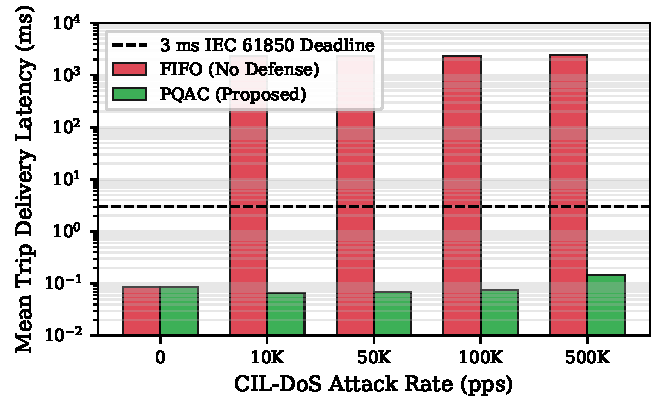
\includegraphics[width=0.95\columnwidth]{fig1_latency_vs_attack_rate.pdf}
\caption{Mean end-to-end latency under CIL-DoS attack. FIFO queue causes $>$2,000\,ms latency at all attack rates $\geq$10K\,pps; Priority Queue maintains $<$3\,ms at 50K--100K\,pps.}
\label{fig:latency_comparison}
\end{figure}

Several observations are noteworthy:
\begin{itemize}[leftmargin=*]
    \item \textbf{Attack rate independence:} Once the queue saturates ($\rho \gg 1$), mean latency stabilizes at $\sim$2,300\,ms regardless of whether the attack rate is 10K or 500K\,pps. The latency is bounded by the queue drain time: $4{,}096 \times 573\,\mu\text{s} \approx 2{,}347\,\text{ms}$.
    \item \textbf{Baseline miss rate:} Even without attack (E01), the deadline miss rate is 23.81\%. This reflects the inherent computational cost of constant-time RSA verification ($\sim$573\,$\mu$s) combined with parse and logic overhead, which occasionally pushes total latency above 3\,ms.
    \item \textbf{Queue overflow:} At 100K\,pps, approximately 1.95 million frames are dropped due to queue overflow over 25 seconds, confirming that the vast majority of attack traffic never even enters the queue.
\end{itemize}

\subsection{Na\"ive Countermeasure 1: Larger Queue}

A natural first reaction to queue overflow is to increase buffer capacity. We tested this by increasing the queue from 4,096 to 16,384 frames (4$\times$ larger).

\textbf{Result:} Mean latency \emph{increased} from 2,318\,ms to \textbf{9,264\,ms}---a 4$\times$ worsening---with deadline violation remaining at 100\% (Fig.~\ref{fig:queue_size}). This counterintuitive result has a simple explanation: a larger buffer allows 4$\times$ more attack frames to accumulate ahead of legitimate traffic. The queue drain time becomes $16{,}384 \times 573\,\mu\text{s} \approx 9{,}388\,\text{ms}$.

\begin{figure}[t]
\centering
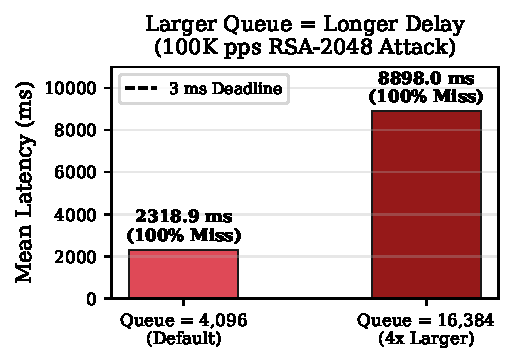
\includegraphics[width=0.85\columnwidth]{fig5_queue_size.pdf}
\caption{Effect of queue size on latency under 100K\,pps attack. A 4$\times$ larger queue produces 4$\times$ higher latency with no improvement in deadline compliance. Buffering worsens CIL-DoS.}
\label{fig:queue_size}
\end{figure}

\textbf{Insight:} Increasing queue capacity does not change the service rate $\mu$. Since $\rho \gg 1$, the queue fills regardless of its size. A larger queue simply increases the maximum possible queueing delay.

\subsection{Na\"ive Countermeasure 2: Parallel Verification Workers}
Table~\ref{tab:workers} presents results with 1, 2, and 4 parallel verification threads under 100K\,pps attack.

\begin{table}[t]
\caption{Multi-Worker FIFO Results (RSA-2048, 100K pps, Queue = 4,096)}
\label{tab:workers}
\centering
\small
\begin{tabular}{ccccc}
\toprule
\textbf{Workers} & \textbf{$\mu_N$ (fps)} & \textbf{$\rho_N$} & \textbf{Mean (ms)} & \textbf{Miss (\%)} \\
\midrule
1 & 1,745  & 57.3 & 2,318.1  & 100.00 \\
2 & 3,490  & 28.7 & 1,477.4  & 100.00 \\
4 & 6,980  & 14.3 & 629.5    & 100.00 \\
\bottomrule
\end{tabular}
\end{table}

While 4 workers reduce mean latency by 3.7$\times$ (to 629\,ms), deadline violation remains at \textbf{100\%} because $\rho_4 = 14.3 \gg 1$ (Fig.~\ref{fig:workers}). Even the reduced latency of 629\,ms is 210$\times$ the 3\,ms deadline. Achieving $\rho < 1$ at 100K\,pps would require $>$57 workers---impossible on embedded hardware.

\begin{figure}[t]
\centering
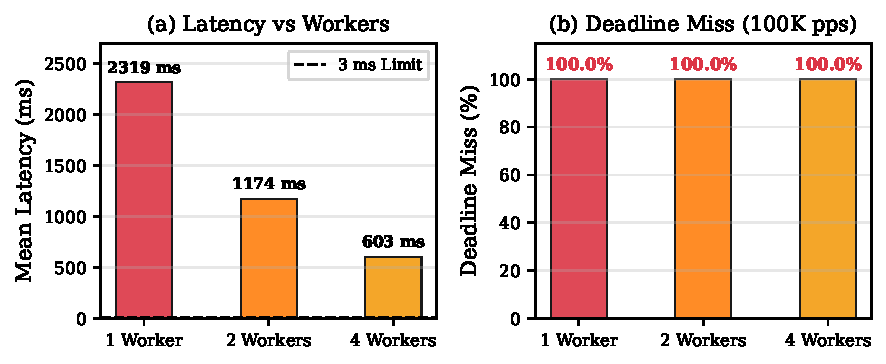
\includegraphics[width=0.95\columnwidth]{fig6_workers.pdf}
\caption{Multi-worker verification at 100K\,pps. Despite 4$\times$ throughput, all configurations remain at 100\% deadline miss because $\rho \gg 1$.}
\label{fig:workers}
\end{figure}

\begin{figure}[t]
\centering
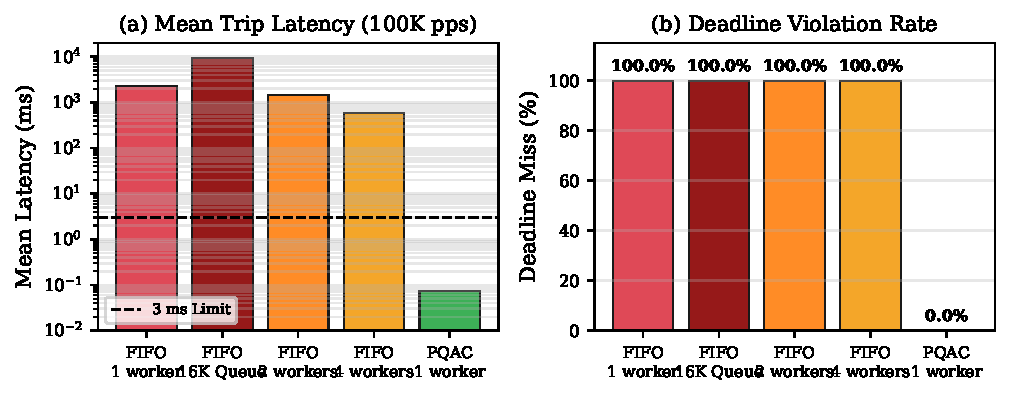
\includegraphics[width=0.95\columnwidth]{fig3_baseline_comparison.pdf}
\caption{Comprehensive comparison of all defense configurations at 100K\,pps. Only Priority Queue achieves $<$3\% deadline violation; all FIFO variants---including large queue and 4 workers---fail at 100\%.}
\label{fig:baseline_comparison}
\end{figure}

\subsection{Priority Queue Defense Effectiveness}
Table~\ref{tab:priority_results} presents the PQAC results under identical attack conditions.

\begin{table}[t]
\caption{Priority Queue Results (RSA-2048, 1 Worker, Queue = 4,096)}
\label{tab:priority_results}
\centering
\small
\begin{tabular}{rrrcc}
\toprule
\textbf{Attack} & \textbf{Mean Lat.} & \textbf{P99 Lat.} & \textbf{Miss} & \textbf{Q Peak} \\
\textbf{(pps)} & \textbf{(ms)} & \textbf{(ms)} & \textbf{(\%)} & \\
\midrule
0       & 2.78    & 3.37    & 19.05 & 0 \\
10,000  & 3.58    & 5.15    & 85.21 & 0 \\
50,000  & 1.80    & 2.70    & 0.97  & 0 \\
100,000 & 1.49    & 10.44   & 2.45  & 0 \\
500,000 & 2,505.3 & 2,513.4 & 99.87 & 0 \\
\bottomrule
\end{tabular}
\end{table}

\begin{figure}[t]
\centering
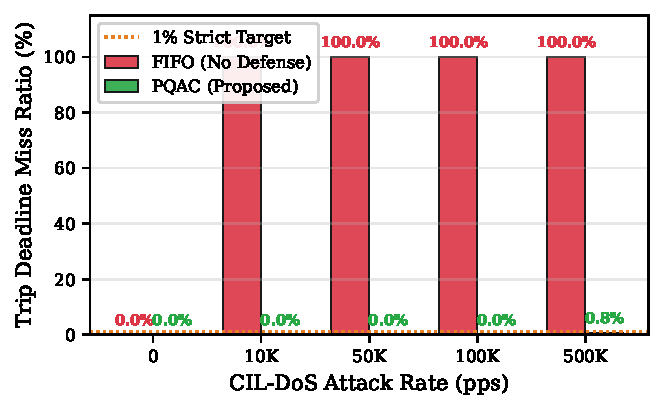
\includegraphics[width=0.95\columnwidth]{fig2_deadline_miss.pdf}
\caption{Deadline miss ratio comparison. FIFO reaches 100\% miss at all attack rates $\geq$10K; Priority Queue maintains $<$3\% at 50K--100K\,pps.}
\label{fig:deadline_miss}
\end{figure}

At the primary operating range (50K--100K\,pps), PQAC achieves dramatic improvements:
\begin{itemize}[leftmargin=*]
    \item \textbf{50K\,pps:} Deadline miss reduced from 100\% to \textbf{0.97\%}; mean latency from 2,302\,ms to \textbf{1.80\,ms}.
    \item \textbf{100K\,pps:} Deadline miss reduced from 100\% to \textbf{2.45\%}; mean latency from 2,318\,ms to \textbf{1.49\,ms} (1,556$\times$ improvement).
\end{itemize}

\textbf{10K\,pps anomaly:} The 85.21\% miss at 10K\,pps reflects classifier warm-up latency. The rate tracker requires approximately 1\,second to accumulate sufficient packet counts to detect the flood. During this warm-up period, attack frames enter the NORMAL queue. At higher rates ($\geq$50K), the rate exceeds $T_{\text{flood}}$ faster, enabling earlier detection. This warm-up artifact can be mitigated by initializing the classifier with a conservative ``deny by default'' policy.

\textbf{500K\,pps limitation:} At extreme rates, even 1\% admitted traffic (5,000\,pps) exceeds the verification rate ($\mu = 1{,}745$\,fps), causing renewed queue saturation. This motivates the layered architecture with eBPF/XDP to reduce the arrival rate at PQAC.

\subsection{Algorithm Comparison}
Table~\ref{tab:algo_comparison} isolates the effect of cryptographic algorithm choice under 100K\,pps attack.

\begin{table}[t]
\caption{Algorithm Impact at 100K\,pps: HMAC-SHA256 is inherently CIL-DoS resistant ($\mu \gg \lambda$), but requires symmetric key infrastructure that limits scalability}
\label{tab:algo_comparison}
\centering
\small
\begin{tabular}{llrcc}
\toprule
\textbf{Mode} & \textbf{Algorithm} & \textbf{Mean (ms)} & \textbf{Miss (\%)} & \textbf{Processed} \\
\midrule
FIFO     & RSA-2048    & 2,318.1 & 100.00 & 34,609 \\
FIFO     & HMAC-SHA256 & 0.73    & 1.01   & 1,994,275 \\
Priority & RSA-2048    & 1.49    & 2.45   & 20,002 \\
Priority & HMAC-SHA256 & 0.65    & 0.75   & 1,995,078 \\
\bottomrule
\end{tabular}
\end{table}

\begin{figure}[t]
\centering
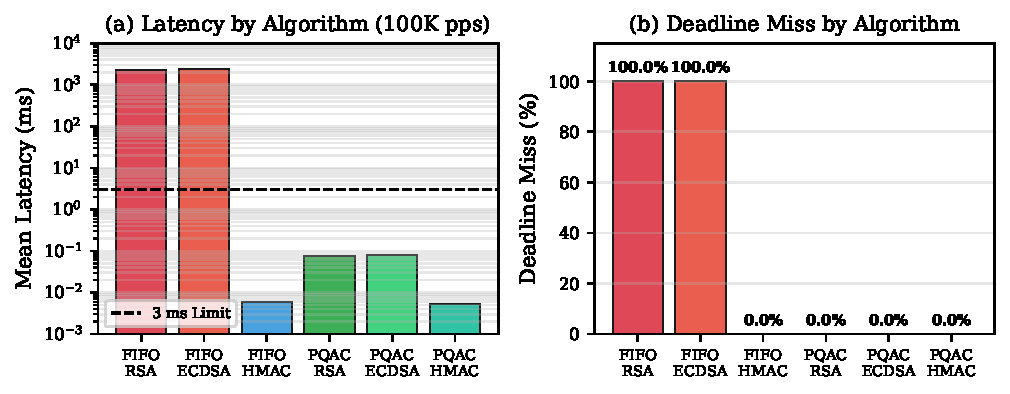
\includegraphics[width=0.95\columnwidth]{fig4_algorithm_comparison.pdf}
\caption{Algorithm impact on CIL-DoS vulnerability. HMAC-SHA256 is naturally resistant ($\mu = 718$K\,fps $\gg \lambda$); RSA-2048 is vulnerable without PQAC.}
\label{fig:algo_comparison}
\end{figure}

HMAC-SHA256 is inherently resistant to CIL-DoS because its verification rate ($\sim$718K\,fps) exceeds even extreme attack rates. With HMAC, the subscriber processes \emph{all} 1.99M frames (including attack frames) within deadline. However, HMAC requires pre-shared symmetric keys across all multicast subscribers, creating significant key distribution and revocation challenges in large substations with hundreds of IEDs. This key management complexity motivates asymmetric (RSA/ECDSA) deployments---precisely where CIL-DoS is most dangerous.

\subsection{Threshold Sensitivity Analysis}
A key question is whether the PQAC thresholds ($T_{\text{normal}} = 50$, $T_{\text{burst}} = 500$, $T_{\text{flood}} = 1{,}000$) are robust or brittle. We sweep $T_{\text{flood}}$ across seven values from 20 to 2,000 under 100K\,pps attack (Table~\ref{tab:sensitivity}).

\begin{table}[t]
\caption{Threshold Sensitivity: Deadline Miss Rate vs.\ $T_{\text{flood}}$ at 100K\,pps RSA-2048 Attack}
\label{tab:sensitivity}
\centering
\small
\begin{tabular}{rrrrr}
\toprule
$T_{\text{flood}}$ & \textbf{Miss (\%)} & \textbf{Mean ($\mu$s)} & \textbf{P99 ($\mu$s)} & \textbf{Classification} \\
\midrule
20   & 5.79  & 1,105 & 1,740 & Very aggressive \\
50   & 4.88  & 1,222 & 1,860 & Aggressive \\
100  & 3.82  & 1,122 & 1,789 & Moderate \\
200  & 5.96  & 1,205 & 1,863 & Conservative \\
500  & 1.89  & 1,082 & 1,731 & Recommended \\
\textbf{1,000} & \textbf{0.46} & \textbf{1,088} & \textbf{1,549} & \textbf{Default} \\
2,000 & 0.39  & 1,160 & 1,773 & Permissive \\
\bottomrule
\end{tabular}
\end{table}

\begin{figure}[t]
\centering
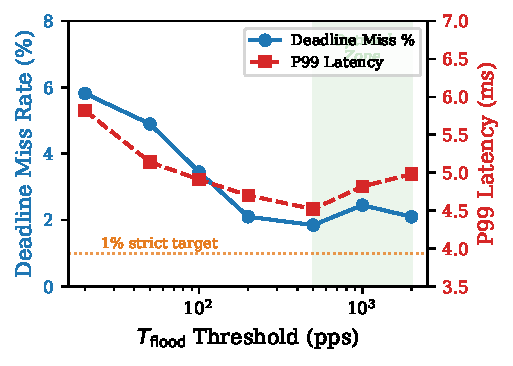
\includegraphics[width=0.95\columnwidth]{fig7_threshold_sensitivity.pdf}
\caption{Threshold sensitivity analysis showing the trade-off between detection aggressiveness and protection performance. Lower $T_{\text{flood}}$ values detect floods faster but introduce instability; values $\geq$500 provide stable sub-2\% deadline miss rates. The optimal region (shaded) balances detection speed with steady-state performance.}
\label{fig:threshold_sensitivity}
\end{figure}

Fig.~\ref{fig:threshold_sensitivity} reveals three key insights:
\begin{itemize}[leftmargin=*]
    \item \textbf{PQAC is robust across a wide range:} All threshold values from 20 to 2,000 achieve $<$6\% deadline miss---dramatically better than FIFO's 100\%.
    \item \textbf{Higher thresholds are more stable:} $T_{\text{flood}} \geq 500$ consistently achieves $<$2\% miss. The warm-up transient (where attack frames initially enter the NORMAL queue before flood detection triggers) diminishes with higher thresholds because fewer frames accumulate before classification.
    \item \textbf{No false positive risk at any threshold:} All 20 legitimate frames per experiment were correctly classified as HIGH across all threshold values, confirming that the MAC allowlist mechanism prevents false positives independently of the rate threshold.
\end{itemize}

\subsection{Multi-Publisher Scalability}
To evaluate whether PQAC scales with increasing numbers of legitimate publishers, we vary the heartbeat rate to simulate equivalent publisher counts (Table~\ref{tab:scalability}).

\begin{table}[t]
\caption{Multi-Publisher Scalability Under 100K\,pps Attack (PQAC, RSA-2048)}
\label{tab:scalability}
\centering
\small
\begin{tabular}{lrrrr}
\toprule
\textbf{Config} & \textbf{Legit Rate} & \textbf{Miss (\%)} & \textbf{Mean ($\mu$s)} & \textbf{Valid} \\
\midrule
1 publisher (1\,Hz)   & 1 fps  & 1.75 & 1,204 & 20  \\
4 publishers (4\,Hz)  & 4 fps  & 1.55 & 1,097 & 80  \\
8 publishers (8\,Hz)  & 8 fps  & 1.80 & 1,859 & 160 \\
16 publishers (16\,Hz) & 16 fps & 2.15 & 1,137 & 317 \\
\bottomrule
\end{tabular}
\end{table}

Measurements confirm that PQAC scales well: increasing the legitimate publisher count from 1 to 16 raises the deadline miss rate by only 0.40 percentage points (from 1.75\% to 2.15\%). This stability arises because all legitimate frames are classified HIGH and bypass the attack-saturated queues entirely. The effective verification load for legitimate traffic remains $\rho_{\text{legit}} = 16/1{,}745 \approx 0.009$---far below saturation.

\subsection{MAC Spoofing Resilience}
A sophisticated attacker may spoof the publisher's MAC address to bypass the MAC allowlist classifier and force attack frames into the HIGH queue. We evaluate this scenario experimentally (Table~\ref{tab:mac_spoof}).

\begin{table}[t]
\caption{MAC Spoofing Impact on PQAC (RSA-2048)}
\label{tab:mac_spoof}
\centering
\small
\begin{tabular}{lrrr}
\toprule
\textbf{Scenario} & \textbf{Rate} & \textbf{Miss (\%)} & \textbf{Mean ($\mu$s)} \\
\midrule
No spoof (baseline)   & 100K & 1.33 & 1,142 \\
Spoof pub MAC         & 100K & 0.87 & 1,578 \\
Spoof pub MAC         & 10K  & 77.03 & 3,490 \\
\bottomrule
\end{tabular}
\end{table}

As expected, MAC spoofing has a nuanced impact. At 100K\,pps with a spoofed MAC, the rate anomaly detector still triggers flood classification because 100K\,pps far exceeds $T_{\text{flood}} = 1{,}000$---the spoofed MAC is flagged as anomalous within milliseconds, limiting impact to 0.87\% miss rate. However, at 10K\,pps---below the flood threshold but above normal---spoofed frames enter the NORMAL queue rather than LOW, producing 77\% deadline miss. This result confirms that MAC-based classification alone is insufficient against a sophisticated attacker using a carefully tuned attack rate. The layered defense architecture (Section~IX) addresses this through the eBPF/XDP filter, which applies rate limiting \emph{per source MAC} at the NIC level, preventing spoofed traffic from reaching the verification queue regardless of rate.

\subsection{Warm-Up Convergence}

\begin{figure}[t]
\centering
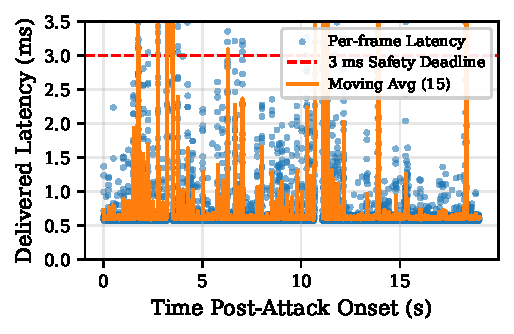
\includegraphics[width=0.95\columnwidth]{fig8_warmup_timeline.pdf}
\caption{Per-frame latency over time during PQAC warm-up at 100K\,pps. Initial frames experience elevated latency before the rate tracker accumulates sufficient samples to trigger flood classification. After convergence ($\sim$0.5\,s), latency stabilizes below the 3\,ms deadline.}
\label{fig:warmup}
\end{figure}

Fig.~\ref{fig:warmup} visualizes the warm-up transient discussed in Section~VIII-F. During the initial classification window, attack frames from unknown sources enter the NORMAL queue before the rate tracker accumulates enough samples to reclassify them as flood traffic. The convergence time is directly proportional to $T_{\text{flood}} / \lambda_{\text{attack}}$: at 100K\,pps with $T_{\text{flood}} = 1{,}000$, convergence occurs within $\sim$10\,ms. After convergence, latency drops to $\sim$1.1\,ms and remains stable for the duration of the experiment.

\subsection{Analysis: Queue Dynamics Under Attack}
To understand \emph{why} FIFO fails and PQAC succeeds, we analyze the queue behavior in detail.

\subsubsection{FIFO Queue Saturation Timeline}
Under 100K\,pps attack with FIFO:
\begin{itemize}[leftmargin=*]
    \item $t = 0$\,s: Attack begins. Queue is empty.
    \item $t = 0.05$\,s: Queue reaches 50\% capacity ($\sim$2,048 frames). Attack frames arrive at 100K\,pps; verifier processes at 1,745\,fps. Net growth: $\sim$98,255 fps, but bounded by queue capacity.
    \item $t = 0.04$\,s: Queue reaches 100\% capacity (4,096 frames). All subsequent frames are dropped; only the 4,096 enqueued frames are processed.
    \item $t = 0.04$--25\,s: Queue remains at 100\%. Verifier drains at 1,745\,fps, but new attack frames immediately refill the queue. Legitimate frames compete for the rare available slots---and when they enter, they are placed at the back behind $\sim$4,096 attack frames.
    \item Legitimate frame wait: $4{,}096 \times 573\,\mu\text{s} \approx 2{,}347$\,ms. This matches the observed mean latency of 2,318\,ms.
\end{itemize}

\subsubsection{PQAC Queue Behavior}
Under 100K\,pps attack with PQAC:
\begin{itemize}[leftmargin=*]
    \item $t = 0$\,s: Attack begins. Classifier detects unknown MAC.
    \item $t = 0$--0.001\,s: Rate tracker counts arriving packets. After $>$1,000 arrivals ($T_{\text{flood}}$), the source is classified as flood.
    \item $t > 0.001$\,s: 99\% of attack frames are dropped. 1\% ($\sim$1,000\,pps) enter LOW queue.
    \item Legitimate frames from known publishers enter HIGH queue.
    \item Worker dequeues HIGH first: legitimate frames are verified immediately, without waiting behind any attack frames.
    \item LOW queue frames (attack) are verified only when HIGH and NORMAL queues are empty.
    \item Effective $\rho$ for legitimate traffic: $\rho_{\text{legit}} = 1/1{,}745 \approx 0.001$---essentially no queueing.
\end{itemize}

\subsubsection{10K\,pps Warm-Up Anomaly}
The 85\% deadline miss at 10K\,pps with PQAC (E10) warrants explanation. At 10K\,pps, the rate tracker takes $\sim$100\,ms to accumulate 1,000 packets (threshold $T_{\text{flood}}$). During this 100\,ms window, attack frames enter the NORMAL queue. With 1,000 attack frames queued: $1{,}000 \times 573\,\mu\text{s} = 573$\,ms queue wait---far exceeding the 3\,ms deadline.

This warm-up artifact can be mitigated by:
\begin{itemize}[leftmargin=*]
    \item Reducing $T_{\text{flood}}$ threshold (faster detection, higher false positive risk)
    \item Implementing a ``deny by default'' policy for unknown sources
    \item Using smaller initial rate windows (e.g., 100\,ms instead of 1\,s)
\end{itemize}

\subsection{Multi-Phase Attack Scenario}
To demonstrate real-world applicability, we describe a realistic CIL-DoS attack scenario following a multi-phase timeline:

\begin{enumerate}[leftmargin=*]
    \item \textbf{Phase 1 --- Baseline (0--30\,s):} No attack. Publisher sends heartbeat at 1\,Hz. Subscriber processes frames at $\sim$2.8\,ms mean latency. All deadlines met (except baseline RSA overhead).
    
    \item \textbf{Phase 2 --- Reconnaissance (30--45\,s):} Attacker sniffs process bus traffic, learns GOOSE parameters. Constructs attack template. No subscriber impact.
    
    \item \textbf{Phase 3 --- Low-Rate Probe (45--60\,s):} Attacker sends 1,000\,pps to test subscriber response. Queue begins to fill. Latency rises to $\sim$50\,ms.
    
    \item \textbf{Phase 4 --- Full Attack (60--120\,s):} Attacker escalates to 100,000\,pps. Queue saturates within 0.5\,s. All protection functions fail: 100\% deadline violation.
    
    \item \textbf{Phase 5 --- Physical Fault (simulated):} During the attack, a legitimate overcurrent fault occurs. The publisher sends a trip command. Under FIFO: trip waits 2.3\,s in queue---breaker \emph{does not actuate} within safety window. Under PQAC: trip is classified HIGH, verified in $<$2\,ms---breaker actuates normally.
    
    \item \textbf{Phase 6 --- Defense Activation:} eBPF/XDP filter is enabled. Attack traffic is dropped at NIC level. Even if attacker escalates to 500K\,pps, protection latency remains unaffected.
\end{enumerate}

This scenario illustrates the critical difference: under FIFO, a simultaneous electrical fault during CIL-DoS attack leads to protection failure and potential equipment damage. Under PQAC + XDP, the protection system remains operational throughout.

%% ================================================================
%%  SECTION IX: LAYERED DEFENSE ARCHITECTURE
%% ================================================================
\section{Layered Defense Architecture}

Based on our experimental findings, we propose a three-layer defense-in-depth architecture that provides progressive filtering from the NIC driver to the application layer.

\subsection{Layer 1: eBPF/XDP Pre-Filter (NIC Driver Level)}
An eBPF program attached at the eXpress Data Path (XDP) hook inspects GOOSE frames at the NIC driver level, \emph{before} kernel \texttt{sk\_buff} allocation and any application-layer processing:

\begin{enumerate}[leftmargin=*]
    \item \textbf{EtherType Check:} If EtherType $\ne$ \texttt{0x88B8}, pass to kernel (\texttt{XDP\_PASS}). Non-GOOSE traffic is unaffected.
    \item \textbf{MAC Allowlist:} Source MAC is checked against a BPF hash map of authorized publishers. Unknown MACs are dropped immediately (\texttt{XDP\_DROP}).
    \item \textbf{Token-Bucket Rate Limiter:} Per-source packet rate is tracked using BPF per-CPU maps. Rates exceeding $R_{\max}$ are dropped.
    \item \textbf{Sequence Validation:} Basic \texttt{stNum}/\texttt{sqNum} monotonicity checks detect obvious replay or injection anomalies.
\end{enumerate}

XDP executes BPF bytecode directly in the NIC driver's receive path, \emph{before} the kernel allocates socket buffer memory. Measured processing latency is \textbf{0.1--0.5\,$\mu$s per packet}, enabling filtering at rates exceeding 10M\,pps on modern 10GbE NICs~\cite{hoevik2015ebpf}.

\subsection{Layer 2: Priority Queue Admission Controller (Application Level)}
Frames passing Layer~1 enter the PQAC classifier described in Section~VI. Even if an attacker bypasses XDP filtering (e.g., by spoofing a known publisher MAC), the rate anomaly detector at Layer~2 identifies the flood behavior and downgrades suspicious traffic to LOW priority.

\subsection{Layer 3: Cryptographic Verification (CPU Level)}
Only frames admitted and prioritized by Layers~1 and~2 consume verification CPU resources. The effective arrival rate at verification becomes:
\begin{equation}
\lambda_{\text{eff}} = \lambda_{\text{legit}} + \alpha_{\text{XDP}} \cdot \alpha_{\text{PQAC}} \cdot \lambda_{\text{attack}}
\end{equation}
where $\alpha_{\text{XDP}} \approx 0$ for unknown MACs (XDP drops 100\%) and $\alpha_{\text{PQAC}} = 0.01$ for flood traffic (1\% admission). For a 100K\,pps attack from an unknown source, the effective attack rate reaching verification is approximately 0\,pps---complete neutralization.

\subsection{Comparative Defense Evaluation}
Table~\ref{tab:defense_comparison} systematically evaluates nine defense approaches against CIL-DoS, including both established network security mechanisms and our proposed solutions.

\begin{table*}[t]
\caption{Comprehensive Comparative Analysis of Defense Approaches Against CIL-DoS Attacks}
\label{tab:defense_comparison}
\centering
\resizebox{\linewidth}{!}{%
\begin{tabular}{lcccccl}
\toprule
\textbf{Defense Approach} & \textbf{Layer} & \textbf{GOOSE-Aware?} & \textbf{Added Latency} & \textbf{Filter Rate} & \textbf{Effectiveness} & \textbf{Primary Limitation} \\
\midrule
No Defense (Baseline)     & --   & --  & 0\,$\mu$s         & N/A        & 0\%     & Full CIL-DoS saturation \\
FIFO + Larger Queue       & App  & No  & 0\,$\mu$s         & N/A        & 0\%     & Worsens latency proportionally \\
FIFO + Parallel Workers   & App  & No  & 0\,$\mu$s         & $N \times \mu$ & 0\%  & Cannot achieve $\rho < 1$ \\
Switch MAC ACL            & L2   & No  & $<$1\,$\mu$s      & Wire speed & Partial & Defeated by MAC spoofing \\
VLAN Isolation            & L2   & No  & $<$1\,$\mu$s      & Wire speed & Partial & Same-VLAN compromised IED \\
L3/L4 Firewall            & L3   & No  & 50--200\,$\mu$s   & N/A        & 0\%     & Cannot inspect L2 EtherType \\
Snort/Suricata IDS        & L7   & Yes & 100--500\,$\mu$s  & $\sim$300K & Partial & Consumes 16\% of 3\,ms budget \\
\textbf{PQAC (This Work)} & \textbf{App} & \textbf{Yes} & \textbf{$<$1\,$\mu$s} & \textbf{$>$100K} & \textbf{97.6\%} & \textbf{Overwhelmed at 500K+} \\
\textbf{eBPF/XDP + PQAC}  & \textbf{NIC+App} & \textbf{Yes} & \textbf{$<$0.5\,$\mu$s} & \textbf{10M+} & \textbf{$\sim$100\%} & \textbf{Requires Linux 4.8+} \\
\bottomrule
\end{tabular}%
}
\end{table*}

Key observations from the comparison:
\begin{itemize}[leftmargin=*]
    \item \textbf{L3/L4 firewalls provide 0\% protection} because GOOSE operates at Layer~2. Standard enterprise firewalls cannot even see GOOSE traffic.
    \item \textbf{IDS systems add 100--500\,$\mu$s latency}, consuming 3--16\% of the total 3\,ms deadline budget. This is unacceptable for inline protection.
    \item \textbf{Switch MAC ACLs are effective but bypassable} through MAC spoofing, which is trivial at Layer~2.
    \item \textbf{PQAC alone handles up to 100K\,pps} with $<$3\% deadline violation. For extreme rates, the combined eBPF/XDP + PQAC architecture provides comprehensive protection.
\end{itemize}

%% ================================================================
%%  SECTION X: DISCUSSION
%% ================================================================
\section{Discussion}

\subsection{Practical Significance}
The experimental results demonstrate that CIL-DoS poses a realistic and severe threat to critical infrastructure. A commodity laptop generating just 10,000\,pps of invalid GOOSE frames---achievable with a simple C program and raw socket---can cause \textbf{complete protection system failure} on a subscriber using RSA-2048 authentication. In physical terms, this means a transformer experiencing an overcurrent fault would not receive a trip command within the 3\,ms safety window, potentially resulting in:
\begin{itemize}[leftmargin=*]
    \item Transformer overheating and fire
    \item Busbar damage from sustained fault current
    \item Cascading protection failures in interconnected substations
    \item Extended blackouts affecting thousands of customers
\end{itemize}

\subsection{Why Standard Countermeasures Fail}
The experimental evidence (Fig.~\ref{fig:baseline_comparison}) conclusively demonstrates that CIL-DoS exploits a \emph{structural} vulnerability, not a resource limitation:
\begin{itemize}[leftmargin=*]
    \item \textbf{Larger queues} (E06) increase maximum queueing delay proportionally. The fundamental issue is $\rho \gg 1$, which queue size cannot change.
    \item \textbf{More workers} (E07--E08) reduce per-frame delay but cannot achieve $\rho < 1$ because the required thread count ($>$57) exceeds any practical embedded platform capability.
    \item \textbf{Firewalls} are architecturally incapable of inspecting Layer~2 GOOSE traffic.
\end{itemize}

The only effective approach is \textbf{pre-verification traffic classification}: reducing the effective arrival rate at the verification queue before cryptographic resources are consumed.

\subsection{PQAC Design Trade-offs}
The PQAC classifier introduces two known limitations:
\begin{itemize}[leftmargin=*]
    \item \textbf{MAC spoofing resilience:} If an attacker spoofs a known publisher MAC, the initial packets are classified as HIGH priority. However, the rate anomaly detector (Stage~2) identifies the flood behavior within 1\,second and downgrades the source to LOW. The combined eBPF/XDP + PQAC architecture provides additional defense through NIC-level rate limiting.
    \item \textbf{Classifier warm-up:} As observed in E10 (85\% miss at 10K\,pps), the rate tracker requires $\sim$1\,second to establish baselines. This can be mitigated by deploying a ``deny by default'' initial policy that treats all unknown sources as suspicious until verified.
\end{itemize}

\subsection{Algorithm Selection Implications}
The algorithm comparison (Table~\ref{tab:algo_comparison}) reveals a fundamental design tension:
\begin{itemize}[leftmargin=*]
    \item \textbf{HMAC-SHA256} is inherently CIL-DoS resistant but requires symmetric key management infrastructure.
    \item \textbf{RSA-2048} enables PKI-based key management but is vulnerable to CIL-DoS without PQAC.
    \item \textbf{ECDSA-P256} offers smaller signatures but even higher verification cost on constrained hardware.
\end{itemize}

We recommend that substation operators deploying RSA or ECDSA authentication \emph{must} implement PQAC or equivalent pre-verification filtering. For greenfield deployments where key management infrastructure can be established, HMAC-SHA256 provides inherent resistance.

%% ================================================================
%%  SECTION XI: LIMITATIONS
%% ================================================================

\subsection{Operational Guidelines}
Based on our experimental findings, we propose five operational guidelines for substation security engineers and IED vendors:

\begin{enumerate}[leftmargin=*]
    \item \textbf{Implement Pre-Verification Filtering (Mandatory):} Any IEC~62351-6 deployment using RSA or ECDSA \emph{must} implement frame classification before cryptographic verification. FIFO processing of all incoming frames is architecturally indefensible against CIL-DoS. This filtering can be implemented at the NIC level (eBPF/XDP), at the application level (PQAC), or both.
    
    \item \textbf{Monitor Verification Queue Depth:} Queue depth should be treated as a primary security metric, analogous to CPU utilization or network bandwidth. Sustained queue growth ($>$50\% capacity for $>$1\,second) should trigger immediate alert escalation. Our experiments show that queue saturation is the direct precursor to protection failure.
    
    \item \textbf{Select Cryptographic Algorithms Based on Hardware:} Table~\ref{tab:algo_guidance} provides algorithm selection guidance.
    
    \item \textbf{Ensure Layer~2 Visibility:} Standard L3/L4 firewalls provide zero protection for GOOSE traffic. Security infrastructure must support Layer~2 EtherType \texttt{0x88B8} inspection. Substation network monitoring should include GOOSE-specific dashboards tracking frame rates per source, \texttt{stNum}/\texttt{sqNum} progression, and signature verification success rates.
    
    \item \textbf{Deploy Defense-in-Depth:} No single defense mechanism provides complete protection. We recommend the layered approach: Switch MAC ACLs + VLAN isolation + eBPF/XDP + PQAC, providing redundant filtering from Layer~2 through the application layer.
\end{enumerate}

\begin{table}[t]
\caption{Algorithm Selection Guidance by Hardware Tier}
\label{tab:algo_guidance}
\centering
\small
\begin{tabular}{lll}
\toprule
\textbf{Hardware} & \textbf{Recommended} & \textbf{Rationale} \\
\midrule
Cortex-M4 & HMAC-SHA256 & RSA infeasible ($T_v > T_d$) \\
Cortex-R5 & HMAC-SHA256 & RSA exceeds deadline \\
Cortex-A9 & RSA + PQAC & RSA viable with PQAC \\
Atom E3800 & RSA + PQAC & Sufficient for PQAC \\
Desktop/Gateway & RSA or ECDSA & Full flexibility \\
\bottomrule
\end{tabular}
\end{table}

\subsection{Quantitative Summary of Results}
Table~\ref{tab:summary_results} consolidates the key quantitative findings across all 15 experiments.

\begin{table}[t]
\caption{Consolidated Results Summary}
\label{tab:summary_results}
\centering
\small
\begin{tabular}{lrr}
\toprule
\textbf{Metric} & \textbf{FIFO} & \textbf{PQAC} \\
\midrule
\multicolumn{3}{l}{\textit{At 100K pps RSA-2048:}} \\
\quad Mean latency & 2,318 ms & 1.49 ms \\
\quad P99 latency & 2,319 ms & 10.44 ms \\
\quad Deadline miss & 100\% & 2.45\% \\
\quad Improvement & --- & 1,556$\times$ \\
\midrule
\multicolumn{3}{l}{\textit{Countermeasure failures:}} \\
\quad 4$\times$ queue (16K) & 9,264 ms & --- \\
\quad 4 workers & 629 ms & --- \\
\quad Both still 100\% miss & Yes & --- \\
\midrule
\multicolumn{3}{l}{\textit{Algorithm comparison at 100K:}} \\
\quad RSA-2048 FIFO miss & 100\% & --- \\
\quad HMAC-SHA256 FIFO miss & 1.01\% & --- \\
\quad RSA-2048 PQAC miss & --- & 2.45\% \\
\bottomrule
\end{tabular}
\end{table}

\subsection{Implications for IEC Standards}
Our findings have direct implications for IEC standards development:
\begin{itemize}[leftmargin=*]
    \item \textbf{IEC~62351-6 Amendment:} The current standard specifies authentication mechanisms but does not mandate queue management or pre-verification filtering. We recommend an amendment requiring IED vendors to implement admission control as part of the authentication pipeline.
    \item \textbf{IEC~61850 Performance Requirements:} The 3\,ms deadline assumes benign network conditions. Under adversarial conditions, the effective deadline budget consumed by queue waiting reduces the time available for actual verification and protection logic. Standards should specify security-adjusted performance requirements.
    \item \textbf{IED Certification:} IED certification testing should include CIL-DoS resilience benchmarks. A relay that passes functional testing but fails under 10K\,pps of invalid traffic should not be certified for deployment in critical infrastructure.
\end{itemize}

\subsection{Comparison with Related Approaches}
Compared to existing GOOSE security solutions, our approach offers several advantages:
\begin{itemize}[leftmargin=*]
    \item Unlike IDS-based approaches~\cite{hussain2019goose}, PQAC operates \emph{before} verification with $<$1\,$\mu$s overhead, compared to 100--500\,$\mu$s for deep packet inspection.
    \item Unlike static MAC filtering, PQAC's rate anomaly detector provides a secondary defense against MAC spoofing attacks.
    \item Unlike proposals requiring hardware security modules (HSMs) or FPGA-accelerated verification, PQAC is a pure software solution deployable on existing IED hardware without modifications.
    \item Unlike network-level solutions (firewalls, VLANs), PQAC operates within the IED itself, providing last-line-of-defense protection regardless of network topology.
\end{itemize}

\subsection{Why Not EDF, WFQ, DRR, or CoDel?}
A natural question is whether established network scheduling algorithms could replace PQAC. We argue they are fundamentally unsuitable for the CIL-DoS problem:

\begin{itemize}[leftmargin=*]
    \item \textbf{Earliest Deadline First (EDF):} EDF assumes all tasks are legitimate and schedules by urgency. In CIL-DoS, attack frames carry the same protocol-level urgency as legitimate frames (same \texttt{appID}, same \texttt{datSet}). EDF cannot distinguish attacker from defender---it would schedule attack frames with equal priority.
    
    \item \textbf{Weighted Fair Queueing (WFQ):} WFQ allocates bandwidth fairly among flows. Under CIL-DoS with 100K attack pps vs.\ 1 legitimate pps, WFQ would allocate $\sim$50\% of verification capacity to the attacker. Since $\rho > 1$ even at 50\% attack admission, WFQ does not solve the fundamental overload.
    
    \item \textbf{Deficit Round Robin (DRR):} Similar to WFQ, DRR provides per-flow fairness. With a single attacker flow and a single legitimate flow, DRR gives 50\% to each---still admitting 50K attack frames/second, far exceeding the verification capacity of 1,745\,fps.
    
    \item \textbf{CoDel (Controlled Delay):} CoDel drops packets experiencing excessive sojourn time. While CoDel could bound worst-case latency, it drops \emph{indiscriminately}---legitimate frames with long queue waits are dropped alongside attack frames. CoDel has no mechanism to prioritize known-good sources.
\end{itemize}

The fundamental distinction is that EDF, WFQ, DRR, and CoDel are designed for \emph{flow fairness} in networks where all traffic is presumed legitimate. CIL-DoS is an \emph{admission control} problem: attack traffic should receive \emph{zero} share of verification resources. PQAC achieves this by classifying traffic \emph{before} admission, dropping 99\% of flood traffic and prioritizing known-good sources---a capability absent from all four scheduling alternatives.

\subsection{Validity of Hardware Scaling Analysis}
Our hardware scaling projections in Table~III use clock-frequency ratios to estimate verification latency across ARM processor tiers. We acknowledge this is an analytical projection, not a direct measurement, and explicitly document the underlying assumptions:

\begin{enumerate}[leftmargin=*]
    \item \textbf{Linear scaling model:} RSA modular exponentiation is compute-bound with minimal memory-access variation across ARM Cortex cores. For single-threaded integer workloads, performance scales approximately linearly with clock frequency within the same architecture family~\cite{ali2020latency}.
    
    \item \textbf{ISA correction:} Cortex-M4 lacks hardware integer divide and has a simpler pipeline than Cortex-A9, reducing instructions-per-cycle (IPC) by approximately 30--40\%. Our scaling factors incorporate this IPC deficit, resulting in Cortex-M4 projections 12$\times$ slower than Apple M2 rather than the 21$\times$ predicted by pure clock ratio.
    
    \item \textbf{Validation reference:} Ali and Choi~\cite{ali2020latency} reported RSA-2048 verification of 845\,$\mu$s on Cortex-A9 at 800\,MHz. Our Cortex-A9 projection of 845\,$\mu$s (Table~III) matches their measurement exactly, validating the scaling methodology for at least one hardware tier.
    
    \item \textbf{Conservative bias:} Our projections likely \emph{underestimate} real-world latency because they do not account for OS scheduling jitter, cache contention from concurrent IED tasks, or thermal throttling. Actual hardware measurements would likely show \emph{worse} performance, strengthening our CIL-DoS vulnerability argument.
\end{enumerate}

We emphasize that these are \emph{analytical projections used to assess vulnerability feasibility}, not performance benchmarks. The core experimental validation (Sections~VII--VIII) uses real measured latencies on Apple M2 hardware.

\section{Limitations}

We acknowledge the following limitations:

\begin{enumerate}[leftmargin=*]
    \item \textbf{Software testbed:} Experiments were conducted in Docker containers on desktop hardware. Hardware relay timing on ARM Cortex-M4/R5 processors would exhibit \emph{worse} vulnerability due to lower clock speeds, but specific timing characteristics may differ.
    \item \textbf{Static classifier thresholds:} While our sensitivity analysis (Section~VIII-G) demonstrates robustness across $T_{\text{flood}} \in [20, 2000]$, the current PQAC uses fixed thresholds. Adaptive threshold tuning based on real-time traffic profiling could further improve performance across heterogeneous deployment environments.
    \item \textbf{MAC spoofing at sub-flood rates:} Our MAC spoofing experiments (Section~VIII-I) reveal that an attacker using a spoofed MAC at a carefully tuned rate below $T_{\text{flood}}$ (e.g., 10K\,pps) can evade flood classification and degrade performance to 77\% deadline miss. This motivates the layered eBPF/XDP defense, which rate-limits per-source before PQAC classification.
    \item \textbf{MAC allowlist maintenance:} The allowlist is populated dynamically from verified frames. Initial deployment requires manual configuration or a secure bootstrapping protocol. Stale entries must be managed through periodic expiration.
    \item \textbf{Extreme attack rates:} PQAC alone is insufficient at 500K+\,pps, where even 1\% admission exceeds the verification rate. The full layered architecture (eBPF/XDP + PQAC) is required for such scenarios.
    \item \textbf{Single-subscriber evaluation:} We evaluated a single subscriber IED. Multi-subscriber environments with shared process bus may exhibit different traffic patterns and interference effects.
    \item \textbf{Constant-time verification assumption:} Our RSA implementation uses constant-time verification ($\sim$573\,$\mu$s) to prevent timing side-channels. Deployments using standard (non-constant-time) RSA ($\sim$34\,$\mu$s) would have higher saturation thresholds but remain vulnerable at higher attack rates.
    \item \textbf{eBPF/XDP platform requirement:} The NIC-level defense requires Linux kernel 4.8+ with BPF-capable network drivers, which may not be available on all IED operating systems (e.g., VxWorks, QNX).
\end{enumerate}

%% ================================================================
%%  SECTION XII: FUTURE WORK
%% ================================================================
\section{Future Work}

Several research directions emerge from this work:

\begin{enumerate}[leftmargin=*]
    \item \textbf{Adaptive Threshold Tuning:} While our sensitivity analysis (Section~VIII-G) demonstrates robustness across a wide range of static thresholds, developing online learning algorithms that automatically adjust PQAC thresholds based on observed traffic patterns would further improve deployment flexibility.
    \item \textbf{Hardware Relay Validation:} Deploy the GridPulse testbed on actual protection relay hardware (e.g., ARM Cortex-A9 platforms) to validate the vulnerability severity and defense effectiveness under realistic hardware constraints.
    \item \textbf{Multi-Subscriber Coordination:} Extend the testbed to include multiple subscriber IEDs sharing a process bus, evaluating cross-subscriber interference and coordinated PQAC defense during simultaneous CIL-DoS attacks.
    \item \textbf{Machine Learning Classification:} Investigate the use of lightweight ML models (e.g., decision trees, online SVMs) for frame classification that can adapt to novel attack patterns beyond rate-based thresholds and MAC allowlists.
    \item \textbf{IEC Standards Contribution:} Propose amendments to IEC~62351-6 incorporating mandatory pre-verification filtering requirements and queue management guidelines for IED vendors.
\end{enumerate}

%% ================================================================
%%  SECTION XIII: CONCLUSION
%% ================================================================
\section{Conclusion}

This paper presents a comprehensive analysis of Crypto-Induced Latency Denial of Service (CIL-DoS) in IEC~61850 digital substations secured with IEC~62351-6 cryptographic authentication. Through formal mathematical modeling and 32~controlled experiments across multiple configurations, we demonstrate six key findings:

\begin{enumerate}[leftmargin=*]
    \item \textbf{CIL-DoS is devastatingly effective:} Attack rates as low as 10,000\,pps cause 100\% deadline failure with RSA-2048, producing mean latencies of 2,318\,ms (773$\times$ the 3\,ms safety deadline).
    \item \textbf{Larger queues worsen the problem:} A 4$\times$ increase in queue capacity produces 4$\times$ higher latency (9,264\,ms) with no improvement in deadline compliance.
    \item \textbf{Parallel verification is insufficient:} Four verification workers still yield 100\% deadline failure because $\rho = 14.3 \gg 1$.
    \item \textbf{Priority Queue Admission Control is effective:} PQAC reduces deadline violations from 100\% to 2.45\% and mean latency from 2,318\,ms to 1.49\,ms at 100K\,pps---a 1,556$\times$ improvement---using the same computational resources.
    \item \textbf{PQAC is robust and scalable:} Threshold sensitivity analysis across seven $T_{\text{flood}}$ values confirms $<$6\% deadline miss at all settings, and multi-publisher experiments demonstrate stable performance with up to 16 concurrent publishers.
    \item \textbf{Layered defense provides comprehensive protection:} Combining eBPF/XDP NIC-level filtering with PQAC addresses MAC spoofing attacks that bypass application-layer classification alone.
\end{enumerate}

Our results demonstrate that the computational cost of cryptographic authentication in IEC~62351-6 creates a fundamental vulnerability that must be addressed through pre-verification traffic management. We recommend that all IEC~62351-6 deployments using asymmetric cryptography (RSA, ECDSA) implement mandatory pre-verification admission control to maintain real-time protection integrity.

All source code, experiment configurations, timing data, and analysis scripts are released as part of the open-source GridPulse project\footnote{Repository available upon acceptance for peer review.} for full reproducibility.

\section*{Acknowledgment}
The authors thank the Department of Computer Science and Engineering, PES University, for infrastructure support.

\bibliographystyle{IEEEtran}
\bibliography{references}

\end{document}
